Sometimes, you want to do something before compiling your tex source files.
For example,
\begin{itemize}
\item Some graphic files are generated with a program like gnuplot.
\item Some tex files are generated with a program like pandoc.
\end{itemize}

Here in this tutorial I want to show you how to use pandoc as a preprocessing program.
Pandoc is a document converter.
It supports many types of format like markdown, latex, html and pdf.
In this tutorial, `Readme.md' in the Buildtools source files is converted to `readme.tex', which is a latex source file.

Most distributions have a pandoc package, so you can install it easily.
If your distribution is ubuntu, type
\begin{verbatim}
$ sudo apt-get install pandoc
\end{verbatim}

To generate `readme.tex', type
\begin{verbatim}
$ pandoc -o readme.tex ../Readme.md
\end{verbatim}

You need to do two more things.
One is changing main.tex and the other is changing helper.tex

First, add {\textbackslash}input command to include readme.tex at the end of main.tex.
\begin{verbatim}
\documentclass{article}
% helper.tex

% You need to rewrite this file to fit your build environment.

% Notice
% The driver of graphicx package is luatex.
% If you use another engine, then you need to rewrite it to your driver.
% For example, if you use pdflatex, then the driver is pdftex.

% Packages
\usepackage{amsmath,amssymb}
\usepackage[luatex]{graphicx}
\usepackage{tikz}
\usetikzlibrary{calc}
\usetikzlibrary{topaths}
\usetikzlibrary{plotmarks}
\usetikzlibrary{intersections}
\usetikzlibrary{arrows,decorations.pathmorphing,backgrounds,positioning,fit,petri}
\usetikzlibrary{arrows.meta}
\usetikzlibrary{3d}

\usepackage{fancybox}
\usepackage{booktabs}

\usepackage[margin=2.4cm]{geometry}

\usepackage[colorlinks=true,linkcolor=black]{hyperref}

% Sample macro.
%\newcommand{\solution}{\begin{flushleft}\textbf{Solution:}\end{flushleft}}
%\newcommand{\proof}{\begin{flushleft}\textbf{Proof}\end{flushleft}}
%\newcommand{\qed}{\begin{flushright}\textbf{q. e. d.}\end{flushright}}
%\newcommand{\answer}[1]{\begin{flushleft}\textbf{Exercise~\ref{#1}}\end{flushleft}}

% Theorem environment.
%\newtheorem{theorem}{Theorem}[section]
%\newtheorem{lemma}{Lemma}[section]
%\newtheorem{corollary}{Corollary}[section]
%\newtheorem{definition}{Definition}[section]
%\newtheorem{example}{Example}[section]
%\newtheorem{exercise}{Exercise}[section]

 ... ...
 ... ...
\section{Make tarball}
  You might want to distribute your source files.
Then, you need to archive them.
The script `arl' looks for the subfiles and the graphics files included by the rootfile, and archive them.
\begin{itemize}
\item If -g option is given, it makes gzip compressed tarball.
\item If -b option is given, it makes bzip2 compressed tarball.
\item If -z option is given, it makes zip file.
\item If no option is given, it makes non-compressed tarball.
\end{itemize}

If some latex source files are generated by preprocessing, you need to generate them before running arl.
\begin{verbatim}
$ arl
$ tar -tf main.tar
main.tex
edit_tex_files.tex
generate_templates.tex
installation.tex
lb.tex
preprocessing.tex
rake.tex
readme.tex
tarball.tex
test_compile.tex
helper.tex
Tutorial_1.png
Tutorial_2.png
hellolatex.png
tableofcontents.png
test_installation.png
\end{verbatim}

Rakefile needs to be added to the tarball.
\begin{verbatim}
$ tar -rf main.tar Rakefile
\end{verbatim}
Then, compress it into gzip.
\begin{verbatim}
$ gzip main.tar
\end{verbatim}

The procedure above is already written in the Rakefile.
Type `rake ar', then rake makes a tarball.
\begin{verbatim}
$ rm main.tar.gz
$ rake ar
arl main.tex
tar -rf main.tar Rakefile
gzip main.tar
mv main.tar.gz Tutorial.tar.gz
\end{verbatim}
Now the name of the tarball is `Tutorial.tar.gz'.

If you want to make a zip file, type `rake zip'.

The tutorial finishes at this section.
Next section is the copy of Readme.md in Buildtools source files.
It describes the background of Buildtools and features of each script.

\hypertarget{buildtools}{%
\section{Buildtools}\label{buildtools}}

\hypertarget{the-background-of-buildtools}{%
\subsection{The background of
Buildtools}\label{the-background-of-buildtools}}

\hypertarget{buildtools-is-a-part-of-latextools}{%
\paragraph{Buildtools is a part of
Latextools}\label{buildtools-is-a-part-of-latextools}}

If you make a long document, for example, a book with more than a
hundred pages, you need to consider various things which isn't necessary
in creating a short document.

\begin{itemize}
\tightlist
\item
  Divide the source file into small parts
\item
  Compile each parts independently
\item
  Replace something with another in the whole document
\item
  Preprocessing (processes before compiling latex source files)
\end{itemize}

Latextools support these things and it includes two parts.

\begin{itemize}
\tightlist
\item
  Buildtools. It is tools which support creating templates of source
  files, building and partial compiling.
\item
  Substools. It is tools which perform replacements in the whole
  document.
\end{itemize}

Buildtools is a part of Latextools and also a core tools in it. This
document describes Buildtools only.

\hypertarget{dividing-a-source-file}{%
\paragraph{Dividing a source file}\label{dividing-a-source-file}}

Latex source files are simply called source files here. It is not
appropriate to write a long document into a single source file. Because,
bigger the file, much more difficult to edit it. To solve this, the
document will be divided into some parts. Usually, they consist of a
file containing \texttt{\textbackslash{}begin\{document\}} and
\texttt{\textbackslash{}end\{document\}} and the other files called by
the file with \texttt{\textbackslash{}include} or
\texttt{\textbackslash{}input} command. The former file is called
rootfile and the latter files are called subfiles. There is a difference
between \texttt{\textbackslash{}include} and
\texttt{\textbackslash{}input} though both are commands to include
subfiles.

\begin{itemize}
\item
  \texttt{\textbackslash{}include} can't be nested. it can be described
  only in the body, which means the part between
  \texttt{\textbackslash{}begin\{document\}} and
  \texttt{\textbackslash{}end\{document\}}.
  \texttt{\textbackslash{}includeonly}, which must be in the preamble,
  specifies a list of files to include by the
  \texttt{\textbackslash{}include} command. The files in the list are
  included by \texttt{\textbackslash{}include} command, and files out of
  the list aren't included even if it is an argument of
  \texttt{\textbackslash{}include} command.
  \texttt{\textbackslash{}include} command issues
  \texttt{\textbackslash{}clearpage} command before and after including
  the file.
\item
  \texttt{\textbackslash{}input} command simply include files. It
  doesn't issue \texttt{\textbackslash{}clearpage} command. This command
  can be nested.
\end{itemize}

It is called build to make a document by compiling. It includes not only
the compilation with latex but also the preprocessing, such as the image
generation by gnuplot or tikz graph generation with data. It is finally
completed by the compilation of the rootfile.

There are several programs to compile LaTeX source files, and they are
called engines. Buildtools supports latex, platex, pdflatex, xelatex and
lualate as engines.

The bigger the document to compile is, the longer the time needs. Even
if you change a small part of the document, it needs the same time as
the big change. You often need to compile to check how the pdf document
looks like, which is sometimes called test, it needs long time in each
compilation. The bigger the document is, the more serious the problem
is. So, it has been thought up to compile a subfile itself without
rootfile or other subfiles.

\begin{itemize}
\tightlist
\item
  Comment out the files in the argument list of
  \texttt{\textbackslash{}includeonly} command which you don't want to
  compile.
\item
  Use subfiles package.
\end{itemize}

Subfiles package is nice and many people recommend it. However, you need
to include the package and use its command appropriately. Naturally, it
is not the matter compared with the compilation time above.

Another way is to add an specific preamble to compile a subfile without
any other files. More specifically, the subfile is put between ``the
text from \texttt{\textbackslash{}documentclass} to
\texttt{\textbackslash{}begin\{document\}}'' and
``\texttt{\textbackslash{}end\{document\}}''. On that occasion, the
subfile itself isn't changed, but another file, which contains the
preamble, \texttt{\textbackslash{}end\{document\}} and
\texttt{\textbackslash{}input} command, is made. The
\texttt{\textbackslash{}input} command reads the subfile. The file newly
made is called ``temporary rootfile''. On the other hand, the rootfile
is sometimes called " original rootfile". The preamble in the temporary
rootfile is a copy of the preamble in the original rootfile. The good
point of this way is:

\begin{itemize}
\tightlist
\item
  There's no need to include any packages or put any special commands.
\item
  Therefore, users don't need to install any packages when the source
  file is distributed.
\end{itemize}

The point is subfile can be compiled separately without any modification
in the source files. The generation of the temporary rootfile is the
only necessary. Buildtools has \texttt{ttex} shell script to do that.

\hypertarget{repeating-compiling}{%
\paragraph{Repeating compiling}\label{repeating-compiling}}

It often needs to compile source files two times or more because of the
cross-reference. The repeating times are maybe two or three (or more),
but I don't know the details. However, there's a great software that
calculate the repeating times automatically. It is latexmk. Latexmk make
the build very easy. Buildtools uses latexmk to compile rootfiles.

\hypertarget{build-directory}{%
\paragraph{Build directory}\label{build-directory}}

Some people might complain about latex because it generates various of
auxiliary files and log files. If you make a build directory and put all
the generated files into it, the source directory can be kept clean. One
of such program is cluttex and it is recommended to people who like
cleanliness.

Buildtools makes a temporary directory, which is also called build
directory, and put all the temporary files and generated document. The
default name of the directory is \texttt{\_build}. It makes the source
directory keep clean. If you want to see log or auxiliary files, search
the build directory for them. It's very simple. Although it is
superfluous to say so, meson build system which is very popular as a C
build tool also uses build directory. This shows us that separating
build directory from source directory is very easy to understand.

Lb, one of the tools in Buildtools, generate a final pdf document in the
build directory. However, many users probably want to put it in the
source directory. It is a natural idea. If you want to do so, use make
or rake.

Rake is a similar program to make. Its advantage is using ruby language
in the Rakefile, which is the script file of rake. Because ruby language
is very strong and flexible, the script file can be readable and
structured.

To get back to the subject how to put a final pdf document in the source
directory, you just write a cp command in your Makefile or Rakefile to
copy the pdf document under the build directory into source directory.
Furthermore, the advantage to use make or rake is that it's possible to
specify preprocessing code in the Makefile or Rakefile. Because
preprocessing depends on the document and what tools the user choose,
it's difficult for Buildtools to cover the preprocessing. Compared with
that, Makefile or Rakefile are really flexible so that you can write
your own preprocessing in it.

It is recommended that users should use make or rake with Buildtools.

\hypertarget{combination-with-texworks}{%
\paragraph{combination with Texworks}\label{combination-with-texworks}}

Lb, one of the tools in Buildtools, can either compile a rootfile or
test-compile a subfile. If you specify it into proccessing tools in the
texworks dialog, you can run lb from texworks and it's so convenient.
Click edit, preference, then typesetting tab. Click plus button in the
processing tools part, then put \texttt{lb}, \texttt{lb},
\texttt{\$fullname} in name, program and arguments box respectively.
Once you set it, you can compile a rootfile or test-compile a subfile by
clicking on the typesetting icon (green triangle icon).

\hypertarget{buildtools-structure}{%
\subsection{Buildtools structure}\label{buildtools-structure}}

Buildtools is made up of the following five parts.

\begin{itemize}
\tightlist
\item
  \texttt{newtex}: It generates source file templates. This is used at
  the beginning of making documents.
\item
  \texttt{lb}: It calls latexmk or ttex to compile source files.
\item
  \texttt{arl}: It makes an archive file.
\item
  installer
\item
  a group of utilities. They are used by the tools above.
\end{itemize}

The following shows the steps to build documents.

\begin{enumerate}
\def\labelenumi{\arabic{enumi}.}
\tightlist
\item
  Make the structure, especially the chapters/sections, of the
  document..
\item
  Run newtex and make folders and templates of the document.
\item
  Modify the templates of Makefile, Rakefile, cover page (cover.tex) and
  preamble (cover.tex) if necessary.
\item
  Write the body of the document and test-compile.
\item
  If necessary, make script files for the preprocessing.
\item
  Compile the rootfile to generate the final pdf document.
\end{enumerate}

The step three to five above are usually repeated and the process is not
necessarily in the order above.

\hypertarget{main-tools}{%
\subsection{Main tools}\label{main-tools}}

Each tool shows its help message if it is run with \texttt{-\/-help}
option. For example, newtex shows the following message.

\begin{verbatim}
$ newtex --help
Usage:
  newtex --help
    Show this message.
  Newtex.conf needs to be edited before running newtex.
  newtex
    A directory is made and some template files are generated under the directory.
\end{verbatim}

The document of each tool is:

\begin{itemize}
\tightlist
\item
  The help message shown by each command with \texttt{-\/-help} option.
\item
  The description below in this document.
\end{itemize}

No other document exists. If you want to know more, see the source code.
All the tools in Buildtools are shell scripts. If you are familiar to
shell scripts, you can easily understand them because they are short.

\hypertarget{newtex}{%
\paragraph{newtex}\label{newtex}}

\begin{verbatim}
$ newtex
\end{verbatim}

Newtex is used when you make a new latex document. irst, decide the
structure and chapters and make \texttt{newtex.conf} in advance. This
script makes a directory and generates template files according to
\texttt{newtex.conf}.

\begin{enumerate}
\def\labelenumi{\arabic{enumi}.}
\tightlist
\item
  There is \texttt{newtex.conf} file in the Buildtools source files.
  Modify it to fit your environment and tex source files you will make.
\item
  Execute \texttt{newtex}. Then it make a directory which name is the
  same as \texttt{title} in \texttt{newtex.conf}. However, the space
  characters in the value of \texttt{title} is converted to underscore
  in the name of the directory. The script also generates template files
  under the directory.
\end{enumerate}

\hypertarget{lb}{%
\paragraph{lb}\label{lb}}

\begin{verbatim}
$ lb [LaTeXfile]
\end{verbatim}

If the argument is left out, \texttt{lb} behaves as if \texttt{main.tex}
is specified as an argument. \texttt{Lb} is a script to build LaTeX
source files and you usually don't need anything except it.

\begin{itemize}
\tightlist
\item
  If the argument is rootfile, then \texttt{lb} compiles it with
  \texttt{latexmk}. If the argument is subfile, then \texttt{lb} runs
  \texttt{ttex} specifying the subfile as an argument.
\item
  If the argument is rootfile, \texttt{lb} compiles it without synctex.
\item
  If the argument is subfile, \texttt{lb} runs \texttt{ttex} and
  \texttt{ttex} compiles the subfile with synctex. After compilation,
  \texttt{lb} runs previewer specified in \texttt{lb.conf}.
\item
  If there exists \texttt{lb.conf} in the current directory (it usually
  contains the rootfile), \texttt{lb} reads it and initialize some
  variables.
\item
  If the variable \texttt{engine} in \texttt{lb.conf} is null string,
  then \texttt{lb} guesses an appropriate engine by itself. However, it
  is recommended that you should specify the engine in \texttt{lb.conf}.
\end{itemize}

You can specify the default values in \texttt{lb.conf} to initialize
some variables.

\begin{verbatim}
rootfile=main.tex
builddir=_build
engine=
latex_option=-halt-on-error
preview=texworks
\end{verbatim}

\begin{itemize}
\tightlist
\item
  \texttt{rootfile} is the name of the rootfile. If you specify the name
  of the rootfile as an argument to \texttt{lb}, then the argument takes
  precedence.
\item
  \texttt{builddir} is the name of the build directory. Auxiliary files
  and output files are put in the build directory. If the argument of
  \texttt{lb} is a subfile, then the temporary rootfile is also put in
  the build directory. If \texttt{builddir} is empty, then no temporary
  directory is generated and the source file directory becomes a build
  directory.
\item
  \texttt{engine} is the name of a latex engine. \texttt{latex},
  \texttt{platex}, \texttt{pdflatex}, \texttt{xelatex} and
  \texttt{lualatex} can be specified. Other engines are not supported.
\item
  \texttt{latex\_option} is a list of options to specify as an argument
  to the engine through \texttt{latexmk}. \texttt{-output-directory} is
  automatically given to \texttt{latexmk} by \texttt{lb} even if
  \texttt{lb.conf}doesn't exist.
\item
  \texttt{preview} is the name of a pdf previewer to show the document.
  It is run only if the argument of \texttt{lb} is a subfile.
\end{itemize}

\hypertarget{arl}{%
\paragraph{arl}\label{arl}}

\$ arl {[}-b\textbar{}-g\textbar{}-z{]} {[}rootfile{]}

The name \texttt{arl} comes from ``ARchive LaTeX files''. It searches
the rootfile for its related files (refer the following) and make an
archive file. If the argument is left out, then it runs as if
\texttt{main.tex} is specified as an argument.

\begin{itemize}
\tightlist
\item
  If there are preprocessing programs, you need to execute them before
  running arl.
\item
  Arl archives the latex source files and the graphic files included by
  \texttt{\textbackslash{}includegraphics} command.
\item
  Therefore, \texttt{Makefile} or the preprocessing script files are not
  archived.
\end{itemize}

It is a good way to make a target (for example, its name is `ar') in
Makefile and write a recipe to add Makefile and the preprocessing files
into the archive file made by \texttt{arl}. You can do the same thing
with Rakefile.

There are options \texttt{-g}, \texttt{-b} and \texttt{-z} to compress
the archive file into \texttt{tar.gz}, \texttt{tar.bz2} and \texttt{zip}
file respectively. If no option is given, \texttt{arl} just make a
tarball without compression.

\hypertarget{utilities}{%
\paragraph{Utilities}\label{utilities}}

You don't need to read this subsection except maintaining the scripts.

\begin{verbatim}
$ srf subfile
\end{verbatim}

This script \texttt{srf} searches for the rootfile of the given subfile
and outputs its absolute path. \texttt{srf} comes from ``Search for Root
File''.

\begin{verbatim}
$ tfiles [-p|-a|-i] [rootfile]
\end{verbatim}

It outputs a list of subfiles of the given rootfile. If the argument is
left out, then it is run as if \texttt{main.tex} is specified as an
argument.

\begin{itemize}
\tightlist
\item
  No option: It outputs a list of subfiles, specified from
  \texttt{\textbackslash{}begin\{document\}} to
  \texttt{\textbackslash{}end\{document\}}. They are the arguments of
  \texttt{\textbackslash{}include} or \texttt{\textbackslash{}input}
  command.
\item
  \texttt{-p}: It outputs a list of subfiles specified with the
  \texttt{\textbackslash{}input} commands in the preamble of the
  rootfile.
\item
  \texttt{-a}: It outputs a list, outputted with no option, and the
  rootfile itself.
\item
  \texttt{-i}: It outputs a list of subfiles specified with both
  \texttt{\textbackslash{}include} and
  \texttt{\textbackslash{}includeonly} command.
\end{itemize}

The files in the list are separated with new lines.

\begin{verbatim}
$ tftype [-r|-s|-q] files ...
\end{verbatim}

It outputs or returns the type of the given latex files.

\begin{itemize}
\tightlist
\item
  \texttt{-r}: It outputs rootfiles which is in the argument files. If
  no options are given, It behaves as if this option is specified.
\item
  \texttt{-s}: It outputs subfiles which is in the argument files.
\item
  \texttt{-q}: It doesn't output anything. The number of the argument
  must be one. It returns an exit status code of the file type. If the
  code is 0 or 1, then the file is a rootfile or subfile respectively.
  Otherwise an error happens.
\end{itemize}

Using \texttt{-q} option is the most common.

\begin{verbatim}
$ gfiles files ...
\end{verbatim}

The argument is a list of latex source files. It outputs graphic files
which are included by \texttt{\textbackslash{}includegraphics} commands
in the given files.

\begin{verbatim}
$ ltxengine rootfile
\end{verbatim}

It guesses a latex engine to compile the rootfile, although it is
recommended that the engine should be specified by the user. For
example,

\begin{verbatim}
\usepackage[luatex]{graphicx}
\end{verbatim}

If this command exists in the preamble, it guesses that the engine is
probably lualatex.

\begin{verbatim}
$ ttex [-b builddir] -e latex_engine [-p dvipdf] [-v previewr] -r rootfile subfile
\end{verbatim}

It generates a temporary rootfile of the subfile and compile it. The
compilation is done only once. Therefore, no cross-reference is carried
out. This comes from the idea that \texttt{ttex} is a script for test to
see how the pdf file looks like and cross-reference is not so important.
The cross-reference to the other files doesn't work neither. This script
can be run directly on the command line, but usually it is called by
\texttt{lb}. The following shows the options.

\begin{itemize}
\tightlist
\item
  \texttt{-b}: Specify a build directory. The default is
  \texttt{\_build}.
\item
  \texttt{-e}: Specify a latex engine. There is no restriction on the
  engine, but it assumes that latex, platex, pdflatex, xelatex or
  lualatex is specified.
\item
  \texttt{-p}: Specify an application that translates dvi into pdf. This
  is used only when the engine is latex or platex, because they outputs
  a dvi file. The default is dvipdfmx. Other possible application is
  dvipdfm and dvipdf.
\item
  \texttt{-v}: Specify a pdf previewer like evince. If you edit the
  source file with texworks, it is a good idea to specify texworks here.
\item
  \texttt{-r}: Specify the original rootfile.
\end{itemize}

\hypertarget{installation-and-uninstallation}{%
\subsection{Installation and
uninstallation}\label{installation-and-uninstallation}}

\hypertarget{prerequisite}{%
\paragraph{Prerequisite}\label{prerequisite}}

\begin{itemize}
\item
  Linux and bash: It is tested on Debian and Ubuntu. However, it
  probably works on other linux distributions. Bash is required because
  this script includes bash commands.
\item
  LaTeX: There are two options to install LaTeX. One is installing the
  LaTeX applications provided by your distribution. The other is
  installing TexLive.
\item
  make or rake: These applications are not necessarily required to run
  the tools in Buildtools. However, it is recommended that they are used
  under the control of make or rake. You don't need to install both of
  them. Choose one which you like. Make is a traditional build tool
  originally aimed at C compiler. Rake is a build tool similar to make.
  It is one of the ruby application. The advantage to use rake is that
  you can put any ruby codes into Rakefile, which is the script file of
  rake. Generally speaking, Rakefile is easy to understand than
  Makefile.
\end{itemize}

\hypertarget{installation}{%
\paragraph{Installation}\label{installation}}

Use the script install.sh.

\begin{verbatim}
$ bash install.sh
\end{verbatim}

This script installs the executable files into \texttt{\$HOME/bin}.
Debian and Ubuntu adds the directory \texttt{\$HOME/bin} into
\texttt{PATH} environment variable if it exists at the login time. The
script makes the directory \texttt{\$HOME/bin} if it doesn't exist. In
that case, you need to re-login to put the directory into the
\texttt{PATH} environment variable. If you run \texttt{sudo} or
\texttt{su} to become the root user before the installation, the
executable files are put into \texttt{/user/local/bin}.

If your OS is debian, type the following to be the root user.

\begin{verbatim}
$ su -
# bash install.sh
\end{verbatim}

Or if it's ubuntu,

\begin{verbatim}
$ sudo bash install.sh
\end{verbatim}

\hypertarget{uninstallation}{%
\paragraph{Uninstallation}\label{uninstallation}}

Use the script uninstall.sh.

\begin{verbatim}
$ bash uninstall.sh
\end{verbatim}

If you run this as a user, the files under \texttt{\$HOME} are removed.
If you run this as a root, the files under \texttt{/usr/local} are
removed. If your OS is debian, type the following to be the root user.

\begin{verbatim}
$ su -
# bash uninstall.sh
\end{verbatim}

Or if it's ubuntu,

\begin{verbatim}
$ sudo bash uninstall.sh
\end{verbatim}

\hypertarget{licence}{%
\subsection{licence}\label{licence}}

Copyright (C) 2020 ToshioCP (Toshio Sekiya)

Buildtools is free software; you can redistribute it and/or modify it
under the terms of the GNU General Public License as published by the
Free Software Foundation; either version 3 of the License, or (at your
option) any later version.

Buildtools is distributed in the hope that it will be useful, but
WITHOUT ANY WARRANTY; without even the implied warranty of
MERCHANTABILITY or FITNESS FOR A PARTICULAR PURPOSE. See the
\href{https://www.gnu.org/licenses/gpl-3.0.html}{GNU Lesser General
Public License} for more details.

\end{document}
\end{verbatim}
In addition, uncommnet the eighth line to let {\textbackslash}tableofcontents command to work.
\begin{verbatim}
 ... ...
\maketitle
% If you want a table of contents here, uncomment the following
 line.
\tableofcontents
 ... ...
\end{verbatim}

Second, {\textbackslash}tightlist command needs to be defined.
Helper.tex is the best place to define it.
\begin{verbatim}
 ... ...
 ... ...
\providecommand{\tightlist}{%
  \setlength{\itemsep}{0pt}\setlength{\parskip}{0pt}}
 ... ...
 ... ...
\end{verbatim}
This code is extracted from \url{https://github.com/jgm/pandoc-templates/blob/master/default.latex}.

Now you can compile it with rake.
\begin{verbatim}
$ rake
\end{verbatim}

\begin{center}
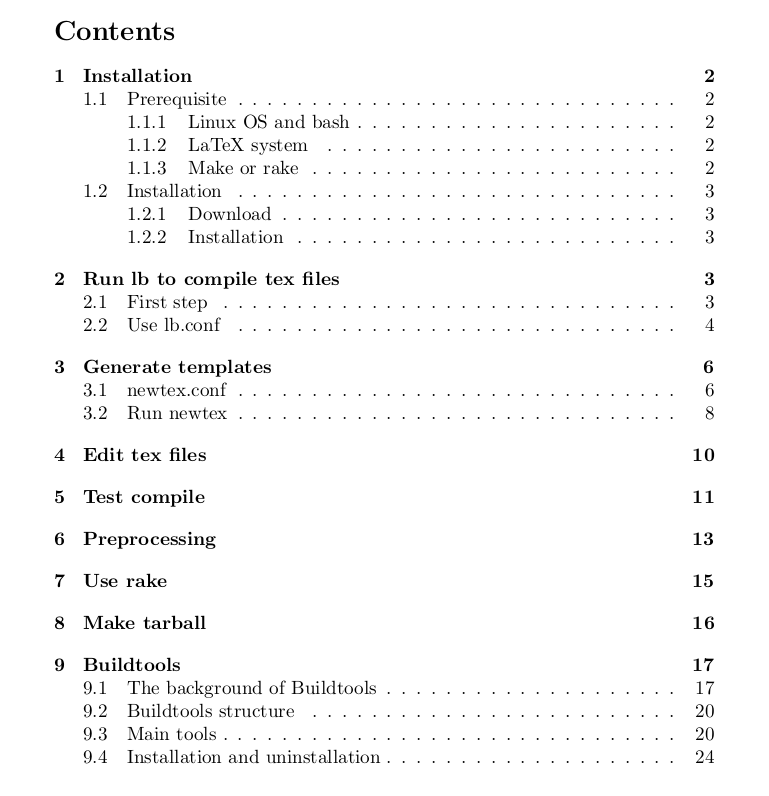
\includegraphics[width=10cm]{tableofcontents.png}
\end{center}

Now the contents of `Readme.md' appears as the section nine in the table of contents.

We ran pandoc by hand in this section.
If Readme.md is upgraded, we need to run pandoc again.
It is a tiresome work and it should be done automatically.
One good way is modify Rakefile so that rake does the preprocessing work automatically before compiling.
It will be shown in the next section.

